\section{Test-and-Fallback in Depth}

The test-and-fallback algorithms are the paper's adaptive robustness
mechanism, and the object of the theory in Section 7. This section gives
their first empirical study: the robustness envelope they achieve
(§5.1), a counter-intuitive failure of the acceptance threshold (§5.2),
its recalibration and the resolution limit that recalibration exposes
(§5.3) --- the empirical face of the budget--stakes law we prove in
Section 7 --- a \textbf{constant-free payoff-testing rule} that the law
suggests and that avoids both threshold pathologies (§5.4), and the
dynamic combiner benchmark that explains \emph{commit-once} (§5.5).
Throughout, the \(\ell_1\) test is the empirical-\(\ell_1\)
proof-of-concept the original authors also fall back to (Section 2.2).

\subsection{The robustness envelope}

We sweep advice error \(\ell_1(p,q)\) on few-types instances
(\(n=2000\), \(r=8\), prefix \(k=200\), 40 trials) and compare blind
FollowPrediction, TestAndMatch (Choo and BEM variants), and the Ranking
floor (\textbf{Figure 2}). The picture is textbook. FollowPrediction
degrades \emph{linearly}, from \(1.000\) at perfect advice to \(0.453\)
at \(\ell_1\!\approx\!1.1\) --- well \emph{below} the advice-free floor
(\(\approx 0.99\)). TestAndMatch instead stays on the \textbf{upper
envelope}: it captures the benefit when advice is good and, when advice
is bad, its prefix test rejects it and it falls back to Ranking. Across
this sweep neither variant gives up more than \(0.02\) against the
advice-free floor, versus FollowPrediction's \(0.54\) (BEM
\(0.998\to0.969\); Choo \(1.000\to0.991\)). That is a statement about
this sweep --- one graph family, 40 trials; the rule-independent version
is Theorem 1. This is the adaptive counterpart of the structural
robustness of Section 3: the engineered mechanism that MPD lacked.

\begin{figure}
\centering
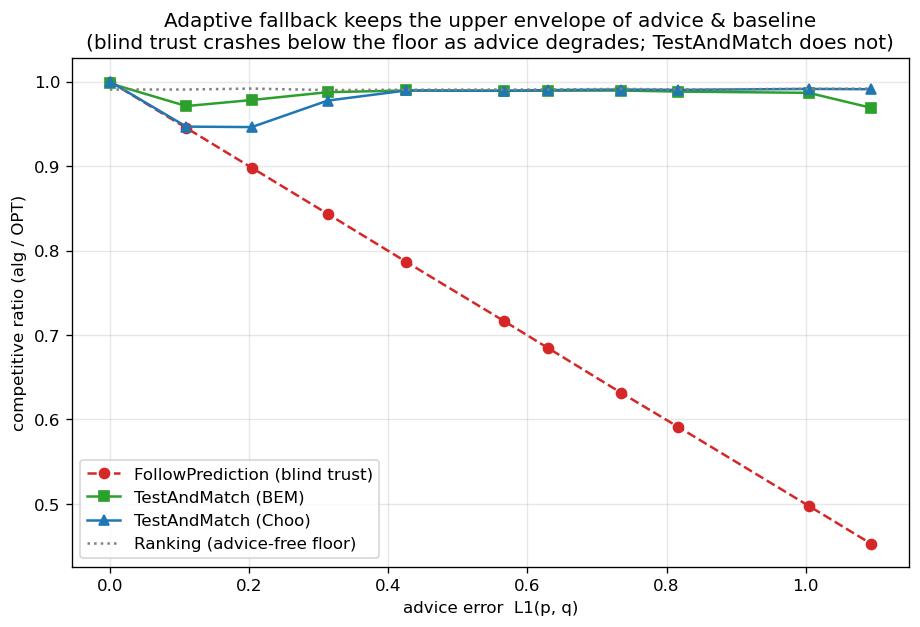
\includegraphics[width=0.7\linewidth,height=\textheight,keepaspectratio,alt={The robustness envelope: blind FollowPrediction crashes below the advice-free floor as advice error grows; TestAndMatch stays on the upper envelope.}]{figs/choo_bem_envelope.png}
\caption{The robustness envelope: blind FollowPrediction crashes below
the advice-free floor as advice error grows; TestAndMatch stays on the
upper envelope.}
\end{figure}

\subsection{A threshold that is too lenient on average-case
inputs}

What does the ``test then maybe fall back'' machinery cost, and does a
better test make a better decision? We sweep the prefix (testing) size
\(k\) at \emph{borderline} advice (\(\eta=0.15\), true
\(\ell_1\!\approx\!0.16\)) --- the regime where the test must work
hardest (\textbf{Figure 3}). Counter-intuitively, \textbf{a larger, more
accurate test makes the \emph{worse} decision}: as \(k\) grows
\(25\to100\to200\to800\), the ratio \emph{falls} \(0.992\to0.981\to
0.969\to0.956\) and the misjudgement rate (against an empirical oracle:
should we have followed, given that following actually underperformed
the baseline here?) \emph{rises} \(0.00\to0.13\to0.33\to0.60\).

\begin{figure}
\centering
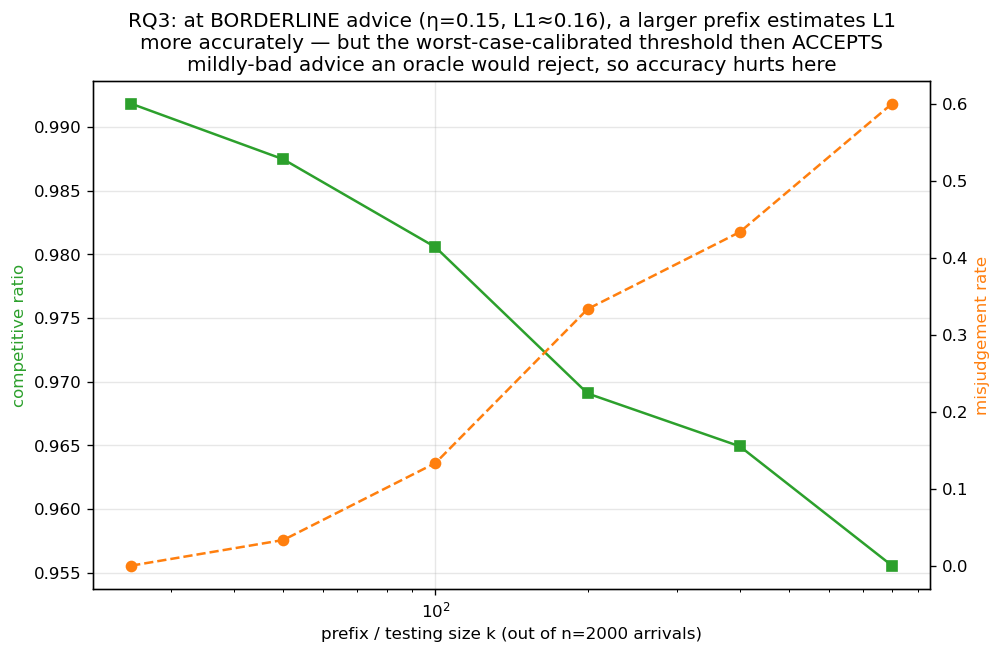
\includegraphics[width=0.7\linewidth,height=\textheight,keepaspectratio,alt={Testing cost at borderline advice: under the worst-case-calibrated threshold, a larger and more accurate prefix test makes the worse decision.}]{figs/choo_bem_prefix.png}
\caption{Testing cost at borderline advice: under the
worst-case-calibrated threshold, a larger and more accurate prefix test
makes the \emph{worse} decision.}
\end{figure}

The mechanism is a real and reportable finding. The Choo/BEM acceptance
threshold \(\tau\) is calibrated to the \emph{worst-case} baseline
\(\beta\approx0.696\) --- the competitive ratio of Ranking under random
arrival order \cite{mahdianyan2011}, and the value Choo et al.~plug into
their threshold \cite{choo2024imperfect}; it is not \(1-1/e\), which is
the adversarial-order guarantee. But on these average-case instances the
baseline is \(\approx0.99\) (Section 3, F3), so the \emph{empirical}
break-even --- the advice error at which following stops beating the
baseline --- sits at \(\ell_1\approx0\), far below \(\tau\). A small,
noisy prefix over-estimates \(\ell_1\) and \emph{accidentally rejects}
the borderline advice, landing on the strong Ranking floor; a large,
accurate prefix correctly measures \(\ell_1\approx0.16<\tau\) and so
\textbf{accepts} the mildly-bad advice the worst-case threshold deems
acceptable --- and underperforms the baseline. On strong-baseline inputs
the worst-case-calibrated threshold is too \emph{lenient}, and improving
the test's accuracy only makes the algorithm follow that miscalibrated
threshold more faithfully.

\subsection{Recalibration, and the resolution limit it
exposes}

The natural fix is to recalibrate \(\tau\) to the \emph{measured}
baseline \(\hat\beta\) (the mean empirical Ranking ratio on a small
calibration sample) rather than the worst-case \(\beta\). On the same
instances this eliminates the pathology: at borderline advice the
worst-case threshold's misjudgement climbs \(0.03\to1.00\) as the prefix
grows and its ratio drops to \(0.920\), whereas the recalibrated
threshold holds misjudgement \(=0.00\) at every prefix size and ratio
\(\approx0.986\) --- a larger prefix no longer hurts.

But recalibration exposes a deeper, honest limit. At \emph{perfect}
advice (\(\ell_1=0\)) the worst-case threshold scores \(1.000\) (it
accepts and follows), while the recalibrated one scores only \(0.987\):
the recalibrated threshold \(\tau\approx 2(1-\hat\beta)\approx 0.028\)
is \emph{smaller than the empirical-\(\ell_1\) estimator's own noise
floor} (\(\approx 0.05\)--\(0.13\) at this prefix and support), so the
test can never confidently \emph{accept} --- it rejects everything,
including perfect advice, and effectively always plays the baseline. In
other words:

\begin{quote}
On strong-baseline instances, no practical empirical-\(\ell_1\)
threshold can both capture the consistency upside and stay safe: the
upside is tiny (the baseline is already \(\approx\mathrm{OPT}\)) and
sits \emph{below the estimator's resolution}. The worst-case threshold
over-accepts (§5.2); the recalibrated threshold over-rejects; and a
better tester only follows whichever threshold more faithfully.
\end{quote}

Section 7 turns this phenomenon into a two-sided law. The resolution
limit above is specific to the empirical-\(\ell_1\) statistic --- §7.7
shows that class is blind for a structural reason (the plug-in distance
saturates at \(k \ll r\) regardless of advice quality) --- but the
deeper point holds for \emph{any} test on a sublinear prefix: the
follow/fallback decision costs a prefix of
\(\tilde\Theta(\sigma^2/g^2)\) --- baseline slack over the square of the
stakes --- and on strong-baseline instances like these the stakes are so
small that the price exceeds the horizon. Section 5 is the empirical
shadow; Section 7 is the law. But the resolution limit is a property of
the \emph{statistic}, not of testing itself --- the next subsection
builds the rule the law suggests, and it behaves differently.

\subsection{Testing the payoff instead: a decision rule with no
constants}

The budget--stakes law identifies the decision-relevant statistic: not
the advice's distance to the truth, but the \emph{payoff} of following
it. We implement this as \textbf{DirectionalTest-and-Match}: the same
commit-once protocol (Mimic the prefix, decide once), with the
\(\ell_1\) threshold replaced by a plug-in payoff comparison. From the
prefix's empirical type distribution \(\hat p\), the value of continuing
to Mimic has an exact closed form,
\(V_{\mathrm{mimic}}(\hat p)=\sum_l \min(n\hat p_l, s_l)\), where
\(s_l\) is the number of offline slots the advice matching allocates to
type \(l\); the value of the Ranking baseline,
\(V_{\mathrm{rank}}(\hat p)\), is estimated by simulating Ranking on the
\emph{public} type graph under the same distribution. The rule follows
iff the corrected difference is nonnegative. Two implementation findings
are part of the paper's message. First, the naive plug-in is
\emph{biased}: \(V_{\mathrm{mimic}}\) is concave, so honest sampling
noise in \(\hat p\) drags the estimate down at the capacity kinks
(Jensen), and an uncorrected rule rejects even perfect advice; a
parametric bootstrap anchored at \(\hat p\) removes the bias (anchoring
at the advice instead over-corrects exactly for mildly bad advice, whose
true distribution sits in the locally linear region). Second, the rule
uses \textbf{no problem constants}: no worst-case \(\beta\), no
threshold \(\tau\) --- every quantity is computed from the prefix and
public information. A public-information early exit (fall back without
spending the prefix when even a \emph{correct} advice would not beat the
baseline) restores parity with Choo et al.'s \(\hat n/n\le\beta\) exit.

\textbf{Figure 4} repeats the envelope sweep with the payoff rule added,
against both the worst-case and the recalibrated thresholds. The three
rules now separate cleanly. At mildly bad advice --- where the
worst-case threshold follows the crash (\(0.948\) and \(0.937\) at
\(\ell_1\approx0.10\) and \(0.21\), misjudging \(100\%\) and \(63\%\) of
instances) --- the payoff rule stays at the floor (\(0.989/0.990\),
misjudgement \(3\%/0\%\)). At perfect advice --- where the recalibrated
threshold \emph{never} follows (misjudgement \(100\%\), §5.3) --- the
payoff rule captures the upside in \({\sim}40\%\) of instances and lands
safely on the floor otherwise. That partial capture is the honest
ceiling, not a defect: at \(k=200\) the family's upside sits \emph{at}
the rule's resolution rather than above it. Rather than assume the
variance, we measured it (\texttt{scripts/measure\_payoff\_variance.py},
Appendix A): drawing prefixes of length \(k\) under perfect advice, the
decision statistic's standard deviation is
\(0.026/0.022/0.019/0.016/0.012\) at \(k=50/100/200/400/800\); holding
the prefix fixed and varying only the simulation seed accounts for under
\(4\%\) of that variance at \(k=200\) and \(k=800\), so these are
sampling numbers. Against this family's stakes (\(g\approx0.02\)) that
is a signal-to-noise ratio of \(1.1\) at \(k=200\) --- precisely the
regime in which a rule follows good advice sometimes and falls back
otherwise. Nor does lengthening the prefix rescue it within the
instance: a \(16\)-fold longer prefix (\(50\to800\)) buys only a
\(2.1\)-fold reduction in noise, leaving the margin at order one across
the entire range we measured. We note one caveat in transferring Section
7 here: \(k\cdot\mathrm{Var}\) is not constant over that sweep
(\(0.033\) to \(0.122\)), so the \(\sigma^2/k\) form proven on the cell
family does not describe this estimator verbatim --- the plug-in is a
kinked functional of the prefix histogram, not a mean of per-sample
observables --- which is why we quote the measurement rather than the
formula. The law's \emph{qualitative} content binds our rule too, and
the right behavior at barely-resolvable stakes is exactly this
safe-either-way coin flip.

\begin{figure}
\centering
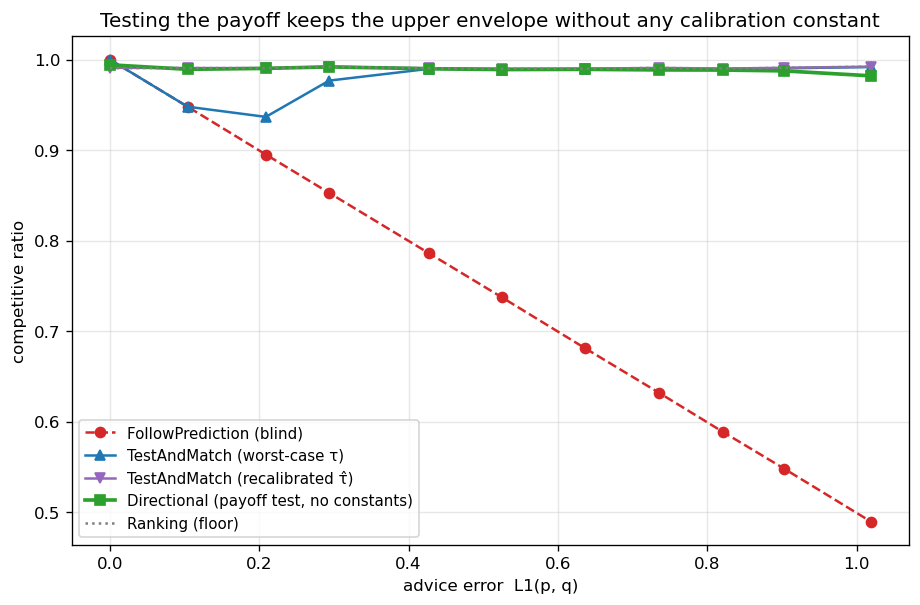
\includegraphics[width=0.85\linewidth,height=\textheight,keepaspectratio,alt={The envelope sweep with the payoff rule added: the worst-case threshold follows the crash at mildly bad advice, the recalibrated threshold never captures at perfect advice, and the constant-free payoff rule tracks the upper envelope within the resolution the budget--stakes law allows.}]{figs/directional_envelope.png}
\caption{The envelope sweep with the payoff rule added: the worst-case
threshold follows the crash at mildly bad advice, the recalibrated
threshold never captures at perfect advice, and the constant-free payoff
rule tracks the upper envelope within the resolution the budget--stakes
law allows.}
\end{figure}

\textbf{Figure 5} is the head-to-head that summarizes the section. At
borderline advice (\(\eta=0.15\)), growing the prefix from \(k=25\) to
\(800\) drives the worst-case threshold's misjudgement \emph{up} from
\(0.07\) to \(1.00\) (ratio \(0.987\to0.922\)) --- §5.2's pathology in
full --- while the payoff rule's misjudgement falls monotonically from
\(0.53\) to \(0.00\) (ratio \(0.954\to0.991\)). More data helps if and
only if the statistic being sharpened is the decision-relevant one; the
recalibrated threshold is flat-safe here only because it always rejects.
In one sentence: \textbf{test the payoff, not the prediction.}

\begin{figure}
\centering
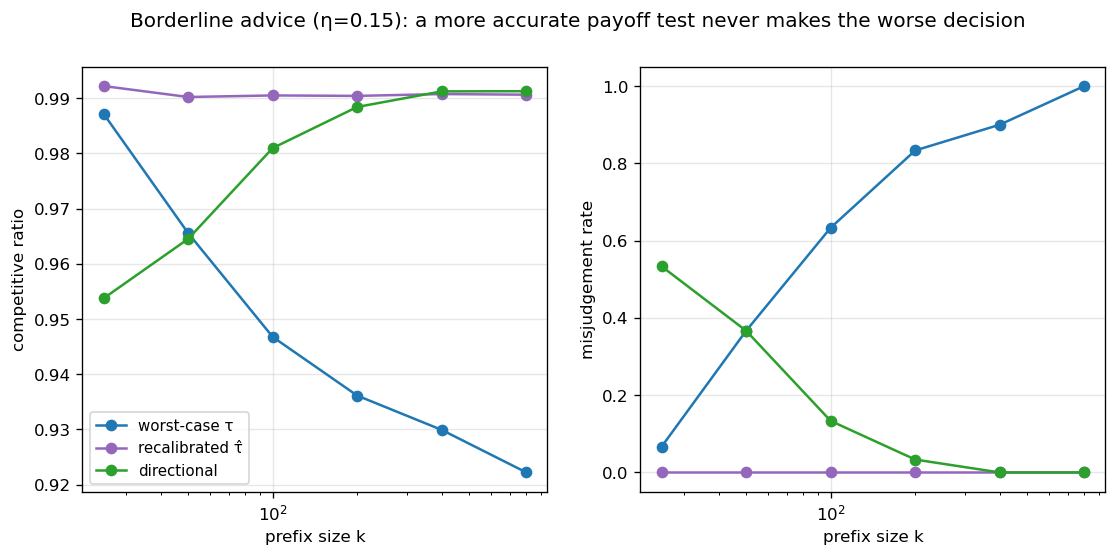
\includegraphics[width=1\linewidth,height=\textheight,keepaspectratio,alt={Borderline advice (\textbackslash eta=0.15): as the prefix grows, the worst-case threshold's misjudgement rises to 1.0 while the payoff rule's falls to 0.0 --- more data helps exactly when the statistic is the decision-relevant one.}]{figs/directional_prefix.png}
\caption{Borderline advice (\(\eta=0.15\)): as the prefix grows, the
worst-case threshold's misjudgement rises to \(1.0\) while the payoff
rule's falls to \(0.0\) --- more data helps exactly when the statistic
is the decision-relevant one.}
\end{figure}

The honest costs: when advice is bad but not worthless-if-true, the
payoff rule pays the same prefix cost as its competitors (\(\approx1\)
point at \(k/n=0.1\); the early exit rarely fires on spiky advice), and
its simulation budget --- a handful of Ranking runs on the type graph
--- is computation, not samples. All numbers: 30 paired trials per
point, seed-fixed (\texttt{scripts/run\_directional\_test.py},
\texttt{results/directional\_test.json}).

\subsection{The dynamic combiner is dominated, and shows why matching
needs
test-then-commit}

Finally we benchmark the Chłędowski-style dynamic combiner (Section 2.2)
to contextualize the \emph{commit-once} structure of test-and-fallback.
In its intended robust tuning the combiner sits exactly on the floor
(\(0.990\) across all advice quality on few-types): it never crashes,
but captures \emph{none} of the consistency upside --- strictly
dominated by TestAndMatch on the good-advice side and equal to it on the
bad side.

More instructively, an \emph{eager} combiner that switches experts
mid-stream reveals a penalty specific to irrevocable problems. On a
single-instance mechanism check (\(n=600\), \(r=6\), one seed, no
averaging --- a demonstration of the mechanism, not a measurement of its
size), eager switching under perfect advice scores \(0.927\),
\emph{below both} the pure follower (\(1.000\)) and the pure baseline
(\(0.958\)), because switching from Ranking to Mimic mid-run lands the
committed matching in an \emph{incompatible hybrid}: the Mimic plan's
slots are already half-consumed by the Ranking phase, and the Ranking
progress is abandoned. In an irrevocable problem the follow/fallback
decision must be made \emph{before} the bulk of the commitments, not
adapted across them --- which is precisely why Choo/BEM test on a prefix
and then \emph{commit}, rather than switching dynamically as the
caching-style combiner does. The dynamic combiner that is cheap
worst-case insurance for caching does not port cleanly to matching, and
the unified benchmark shows why.
